% !TeX root = thesis.tex

\chapter{Related work}
In the previous chapter I have stressed the paramount importance of periodically integrating one's changes into the upstream repository. Additionally, Continuous Integration was introduced as both a practice and a tool to facilitate this often complex and time-consuming process. However, Continuous Integration is not the golden bullet for software engineering. In this chapter I will investigate the flip side of applying this practice. After every integration, all of the unit and regression tests in the test suite must be executed to ensure that the integration was successful and that no new bugs have been introduced. As the project evolves, the size of the codebase increases and consequently the amount of tests will increase as well in order to maintain a sufficiently high coverage level. An increase in the size of the test suite will inevitably lead to an increase in test duration \cite{evaluationoftestsuiteminimization}, which imposes an issue of scaling. Walcott, Soffa and Kapfhammer illustrate the magnitude of this problem by providing an example of a codebase consisting of 20.000 lines, for which the tests require up to seven weeks to complete \cite{10.1145/1146238.1146240}.\\

\noindent Fortunately, multiple developers and researchers have found some techniques that can be used to address the scalability issues of growing test suites. The techniques currently known to literature can be classified in three categories. Developers can either apply \emph{\tsm{}}, \emph{\tcs{}} or \emph{\tcp{}} \cite{evaluationoftestsuiteminimization}. All three techniques are applicable to any test suite, however there is a trade-off to be made. Depending on which technique is chosen, it will either have a major impact on the duration of the test suite execution in exchange for a reduced test coverage level, or it will result in a higher test adequacy.\\

\noindent In the following sections I will first elaborate on the details of these three approaches, then I will provide accompanying algorithms that can be used. Since the approaches share common ideas, the algorithms can (albeit with minor modifications) be reused across all approaches. In the final section I will illustrate some examples of the discussed techniques and algorithms that are currently integrated in existing software testing frameworks.

% !TeX root = ../thesis.tex

\section{Classification of approaches}

% !TeX root = ../../thesis.tex

\subsection{\tsm{}}
\label{ssec:tsm}
The first technique is called \acrfull{tsm}, also referred to as \emph{Test Suite Reduction} in literature. This technique will try to reduce the size of the test suite by permanently removing redundant test cases. This problem has been formally defined by Rothermel \cite{10.1002/stv.430} in \cref{def:tsm} and illustrated in \Cref{fig:tsm}.

\begin{definition}[\tsm{}]
\label{def:tsm}
\mbox{}\\Given:
\begin{itemize}
	\item $T = \{t_1, \dots, t_n\}$ a test suite consisting of test cases $t_j$.
	\item $R = \{r_1, \dots, r_m\}$ a set of requirements that must be satisfied in order to provide the desired ``adequate'' testing of the program.
	\item $\{T_1, \dots, T_m\}$ subsets of test cases in $T$, such that for every $i \in [1..m]$, any one of the test cases $t_j \in T_i$ can be used to satisfy requirement $r_i$.
\end{itemize}

\noindent Subsequently, we can define \tsm{} as the task of finding a subset $T'$ of test cases $t_j \in T$ that satisfies every requirement $r_i$.
\end{definition}

\noindent If we apply the concepts of the previous chapter to the above definition, we can interpret the set of requirements $R$ as source code lines that must be covered. A requirement $r_i$ can subsequently be satisfied by any test case $t_j \in T$ that belongs to the subset $T_i$. Observe that the problem of finding $T'$ is closely related to the \emph{hitting set problem} (\cref{def:hitting-set}) \cite{10.1002/stv.430}.

\begin{definition}[Hitting Set Problem]
\label{def:hitting-set}
\mbox{}\\Given:
\begin{itemize}
	\item $S = \{s_1, \dots, s_n\}$ a finite set of elements.
	\item $C = \{c_1, \dots, c_n\}$ a collection of sets, with $\forall c_i \in C : c_i \subseteq S$.
\end{itemize}

\noindent The hitting set is a subset $S' \subseteq S$ such that $S'$ contains at least one element from each subset in $C$.
\end{definition}

\noindent In the context of \tsm{}, $T'$ corresponds to the hitting set of $T_i$s. In order to effectively minimise the amount of tests in the test suite, $T'$ should be the minimal hitting set \cite{10.1002/stv.430}. Since we can reduce this problem to the NP-complete \emph{Vertex Cover}-problem, we know that this problem is NP-complete as well \cite{10.5555/574848}.

\begin{figure}[htbp!]
	\centering
	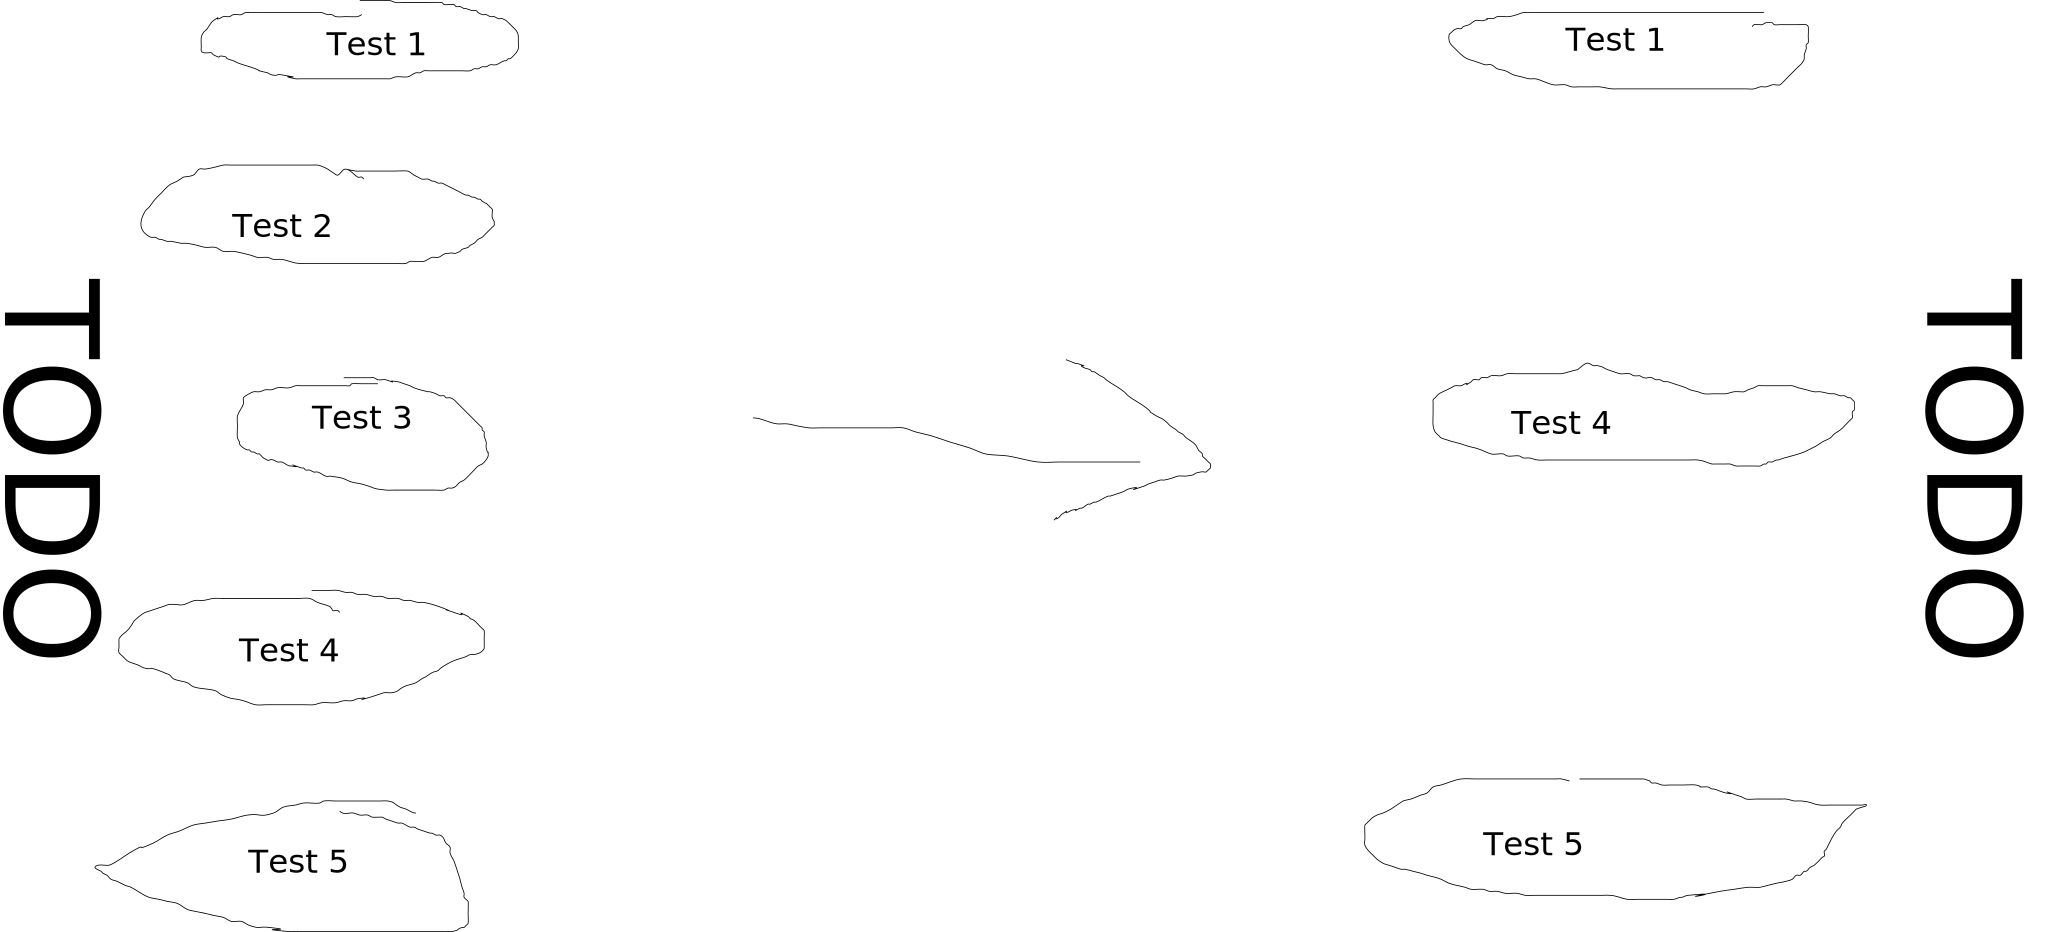
\includegraphics[width=\textwidth]{assets/tikz/approach-tsm.tikz}
	\caption{\tsm{}.}
	\label{fig:tsm}
\end{figure}
% !TeX root = ../../thesis.tex

\subsection{\tcs{}}
The second algorithm closely resembles the previous one. Instead of determining the minimal hitting set of the test suite in order to permanently remove tests, this algorithm has a notion of context. Prior to the execution of the tests, the algorithm performs a \emph{white-box static analysis} of the codebase to identify which parts have been changed. Subsequently, only the tests regarding modified parts are executed, making the selection temporary (\autoref{fig:tcs}) and modification-aware \cite{10.1002/stv.430}. Rothermel and Harrold define this formally in \autoref{def:tcs}.

\begin{definition}[\tcs{}]
\label{def:tcs}
\mbox{}\\Given:
\begin{itemize}
	\item $P$ the previous version of the codebase
	\item $P'$ the current (modified) version of the codebase
	\item $T$ the test suite
\end{itemize}

\noindent \tcs{} aims to find a subset $T' \subseteq T$ that is used to test $P'$. 
\end{definition}

\begin{figure}[htbp!]
	\centering
	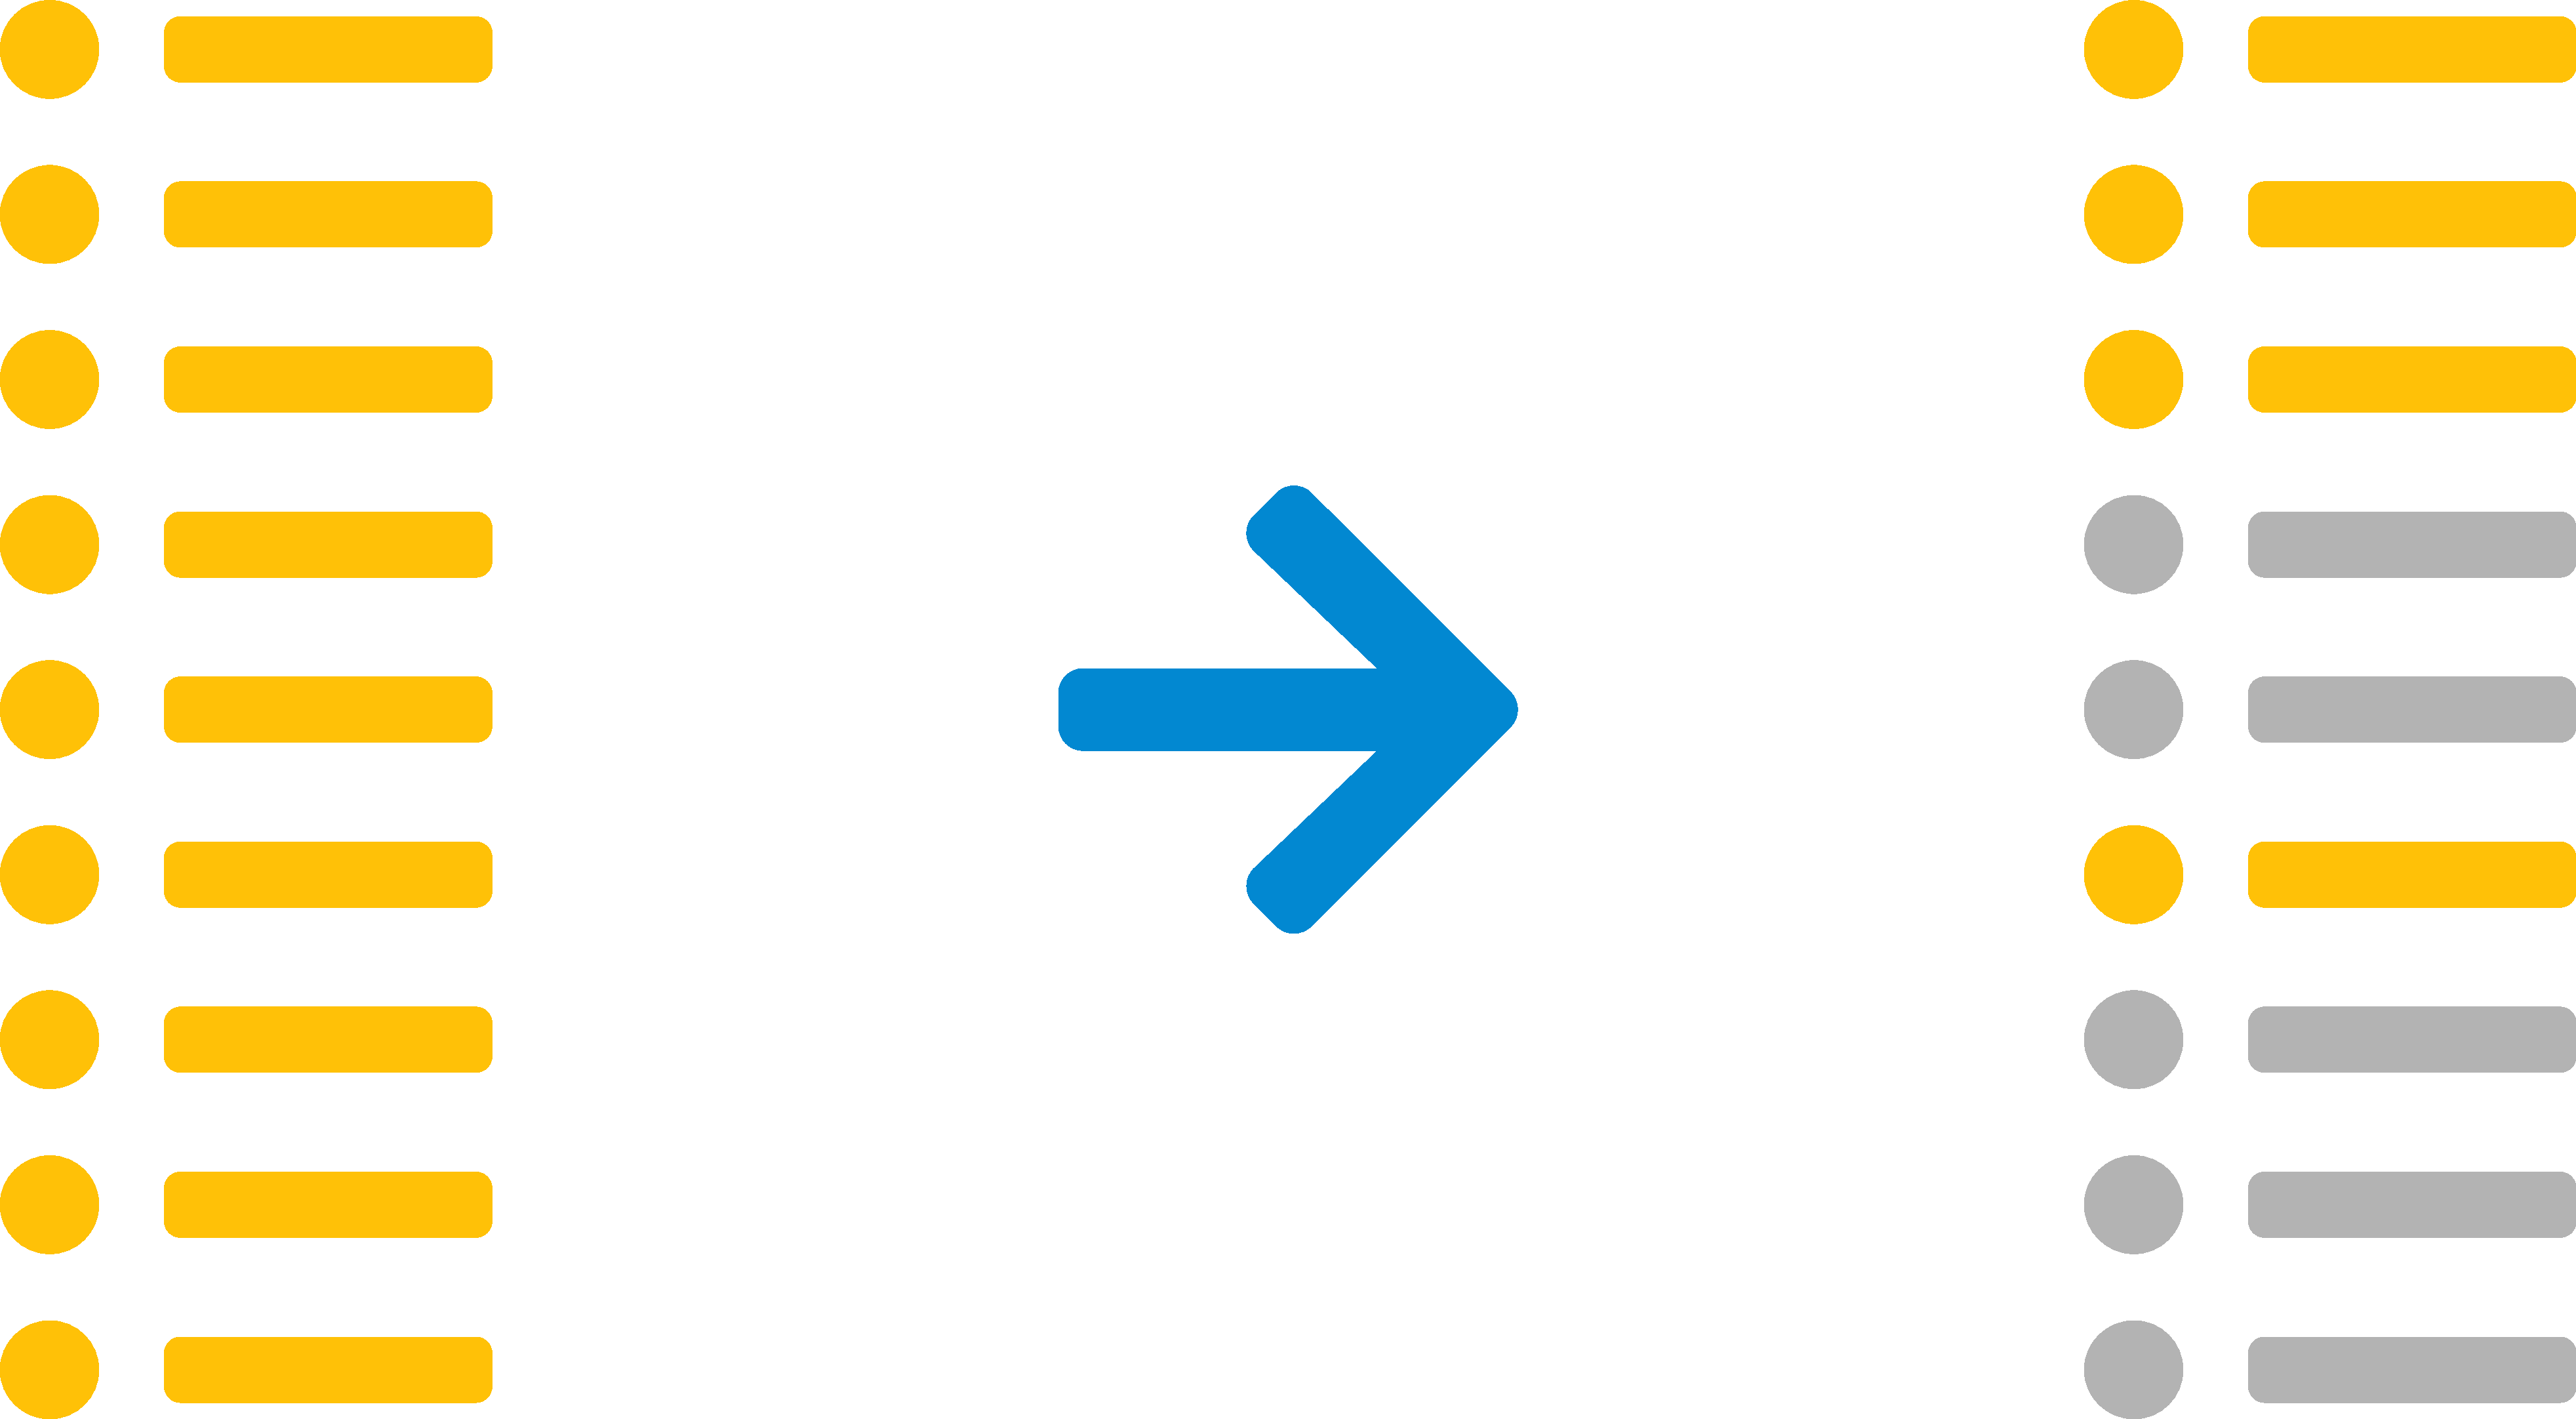
\includegraphics[width=0.8\textwidth]{assets/approach-tcs.pdf}
	\caption{\tcs{}}
	\label{fig:tcs}
\end{figure}
% !TeX root = ../../thesis.tex

\subsection{\tcp{}}
Both \acrshort{tsm} and \acrshort{tcs} attempt to execute as few tests as possible to reduce the execution time of the test suite. Nevertheless, in some cases, we may require to execute every test case to guarantee correctness. In this situation, we can still optimise the test suite. \acrfull{tcp} aims to find a permutation of the sequence of test cases, rather than eliminating specific tests from being executed (\Cref{fig:tcp}). We choose the order of the permutation in such a way that we can complete a predefined objective as soon as possible. Once we have achieved our objective, we can early terminate the execution of the test suite. In the worst-case scenario, we will still execute every test case. Some examples of objectives include covering as many lines of code as fast as possible or executing tests ordered on their probability of failure \cite{10.1002/stv.430}. \Cref{def:tcp} provides a formal definition of this approach.

\begin{definition}[\tcp{}]
\label{def:tcp}
\mbox{}\\Given:
\begin{itemize}
	\item $T$ the test suite
	\item $PT$ the set of permutations of $T$
	\item $f: PT \mapsto \mathbb{R}$ a function from a subset to a real number, this function is used to compare sequences of test cases to find the optimal permutation.
\end{itemize}

\noindent \tcp{} finds a permutation $T' \in PT$ such that $\forall T'' \in PT : f(T') \ge f(T'') \Rightarrow (T'' \ne T')$ 
\end{definition}

\begin{figure}[htbp!]
	\centering
	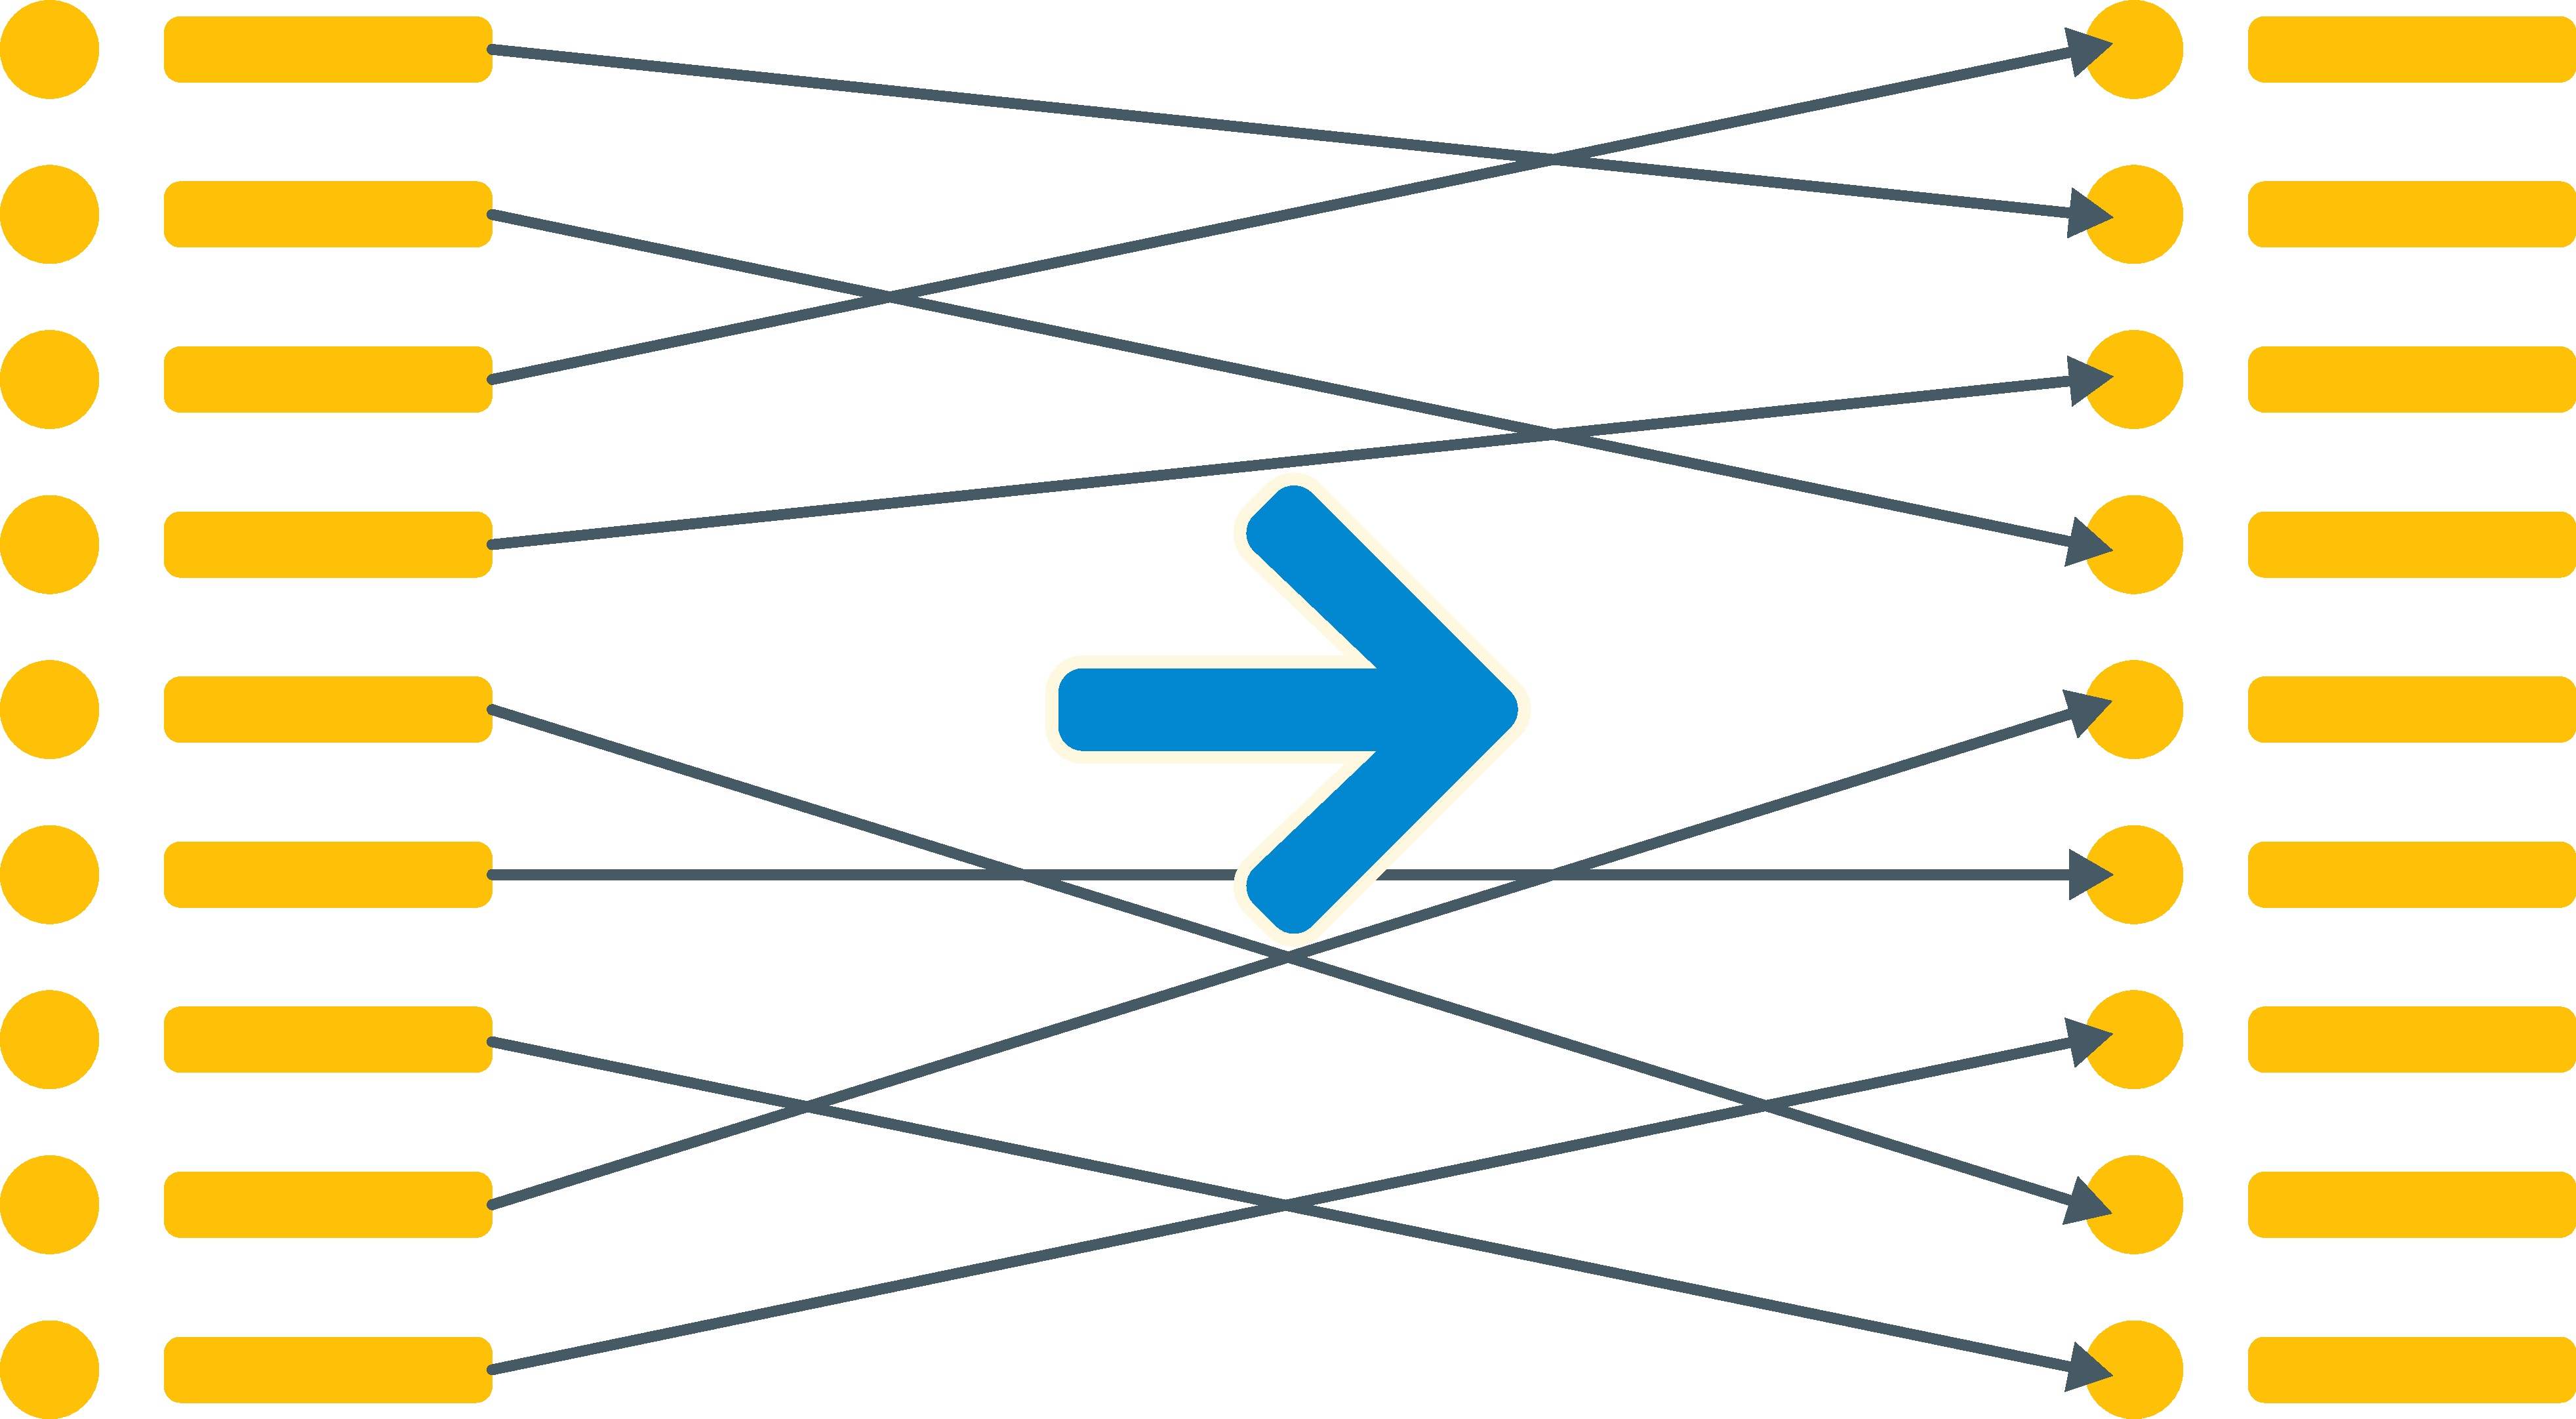
\includegraphics[width=\textwidth]{assets/tikz/approach-tcp.tikz}
	\caption{\tcp{}.}
	\label{fig:tcp}
\end{figure}
% !TeX root = ../thesis.tex

\section{Algorithms}
In \autoref{ssec:tsm} the relation was explained between applying Test Suite Minimisation and finding the minimal hitting set of the test suite and the set of requirements, which is an NP-complete problem. Therefore, the use of \emph{heuristics} is required. A heuristic is an experience-based method that can be used to solve a hard to compute problem by finding a fast approximation \cite{6588537}. However, the found solution will mostly be suboptimal or might sometimes even fail to find any solution at all. Considering its relation to the minimal hitting set problem, heuristics that are known to literature for solving this problem can also be used to implement \tsm{}. A selection of these heuristics will be discussed below. It should be noted however that the used terminology and naming of the variables might have been changed to ensure mutual consistency. Every algorithm has been modified to adhere to the conventions provided in \autoref{def:alg-naming} and \autoref{def:cardinality}.

\begin{definition}[Naming convention]
\label{def:alg-naming}
\mbox{}
\begin{itemize}
	\item $C$: the set of all lines in the application source code that are covered by at least one test case $t \in TS$.
		\begin{itemize}
			\item $CT_l$ denotes the test group $l$, which corresponds to the set of all tests $t \in TS$ that cover source code line $l \in C$.
		\end{itemize}
	\item $RS$: the representative set of test cases, these are the test cases that have been selected by the algorithm.
	\item $TS$: the set of all test cases in the test suite.
		\begin{itemize}
			\item $TL_t$ denotes the set of all source code lines that are covered by test $t \in TS$.
		\end{itemize}
\end{itemize}
\end{definition}

\begin{definition}[Cardinality]
\label{def:cardinality}
For a finite set $S$, the cardinality $|S|$ is defined as the number of elements in $S$. In case of potential confusion, the cardinality of $S$ can also be denoted as $Card(S)$.
\end{definition}

% !TeX root = ../../thesis.tex

\subsection{Greedy algorithm}
\label{ssec:alg-greedy}
The first algorithm is a \emph{greedy} heuristic, which was originally designed by Chvatal to find an approximation for the set-covering problem \cite{evaluationoftestsuiteminimization}. A greedy algorithm always makes a locally optimal choice, assuming that this will eventually lead to a globally optimal solution \cite{10.5555/1614191}. Algorithm \ref{alg:tsm-greedy} presents the Greedy algorithm for \tsm{}. The goal of the algorithm is to construct a set of test cases that cover every line in the code, by requiring as few tests as possible.\\

\noindent Initially, the algorithm starts with an empty result set $RS$, the set $TS$ of all test cases and the set $C$ of all coverable source code lines. Furthermore, $TL_t$ denotes the set of source code lines in $C$ that are covered by test case $t \in TS$. Subsequently, the algorithm iteratively selects test cases from $TS$ and adds them to $RS$. The locally optimal choice is to always select the test case that will contribute the most still uncovered lines, ergo the test $t$ for which the cardinality of the intersection between $C$ and $TL_t$ is maximal. After every iteration, the now covered lines $TL_t$ are removed from $C$ and the selection process is repeated until $C$ is empty. Upon running the tests, only the tests in $RS$ must be executed. This algorithm can be converted to make it applicable to \tcp{} by converting the set $RS$ to a list to maintain the order in which the test cases were selected, which is equivalent to the prioritised order of execution.

\begin{algorithm}[h!]
\caption{Greedy algorithm for \tsm{}}
\label{alg:tsm-greedy}
\begin{algorithmic}[1]
	\State {\bfseries Input:} Set $TS$ of all test cases, set $C$ of all source code lines that are covered by any $t \in TS$ and $TL_t$ the set of all lines are covered by test case $t \in TS$.
	\State {\bfseries Output:} Subset $RS \subseteq TS$ of tests to execute.
	\State $RS \gets \emptyset$
	\While{$C \neq \emptyset$}
		\State $t\_max \gets 0$
		\State $tl\_max \gets \emptyset$
		
		\ForAll{$t \in TS$}
			\State $tl\_current \gets C \cap TL_{t}$
			\If{$|tl\_current| > |tl\_max|$}
				\State $t\_max \gets t$
				\State $tl\_max \gets tl\_current$
			\EndIf
		\EndFor
		
		\State $RS \gets RS \cup \{t\_max\}$
		\State $C \gets C \setminus tl\_max$
	\EndWhile
\end{algorithmic}
\end{algorithm}

% !TeX root = ../../thesis.tex

\subsection{HGS}\label{ssec:alg-hgs}
The second algorithm was created by Harrold, Gupta and Soffa \cite{hgs}. This algorithm constructs the minimal hitting set of the test suite in an iterative fashion. As opposed to the greedy algorithm (\autoref{ssec:alg-greedy}), the HGS algorithm considers the test groups $CT$ instead of the set $TLt$ to obtain a list of test cases that cover all source code lines. More specifically, this algorithm considers the distinct test groups, denoted as $CTD$. Two test groups are considered indistinct if they differ in at least one test case. The pseudocode for this algorithm is provided in Algorithm \autoref{alg:hgs}.\\

\noindent Similar to the previous algorithm, an empty representative set $RS$ is constructed in which the selected test cases will be stored. The algorithm begins by iterating over every source code line $l \in C$ and constructing the corresponding set of test groups $CT_l$. As mentioned before, for performance reasons this set is reduced to $CTD$, only retaining distinct test groups. Next, the algorithm selects every test group of which the cardinality is equal to 1 and adds these to $RS$. This corresponds to every test case that covers a line of code, which is exclusively covered by that single test case. Subsequently, the lines that are covered by any of the selected test cases are removed from $C$. This process is repeated for an incremented cardinality, until every line in $C$ is covered. Since the remaining test groups will now contain more than one test case, the algorithm needs to make a choice on which test case to select. The authors have chosen that the test case that occurs in the most test groups is preferred. In the event of a tie, this choice is deferred until the next iteration.\\

\noindent The authors have provided an accompanying calculation of the computational time complexity of this algorithm \cite{hgs}. With respect to the naming convention introduced in \autoref{def:alg-naming}, additionally let $n$ denote the number of distinct test groups $CTD$, $nt$ the number of test cases $t \in TS$ and $MAX\_CARD$ the cardinality of the largest test group. The HGS algorithm consists of two steps which are performed repeatedly. The first step involves computing the number of occurrences of every test case $t$ in each test group. Given that there are $n$ distinct test groups and, in the worst case scenario, each test group can contain $MAX\_CARD$ test cases which all need to be examined once, the computational cost of this step is equal to $O(n * MAX\_CARD)$. In order to determine which test case should be included in the representative set $RS$, the algorithm needs to find all test cases for which the number of occurrences in all test groups is maximal, which requires at most $O(nt * MAX\_CARD)$. Since every repetition of these two steps adds a test case that belongs to at least one out of $n$ test groups to the representative set, the overall runtime of the algorithm is $O(n * (n + nt) * MAX\_CARD)$.
\begin{algorithm}[h!]
\caption{HGS algorithm (\cite{hgs})}
\label{alg:hgs}
\begin{algorithmic}[1]
	\State {\bfseries Input:} Distinct test groups $T_1, \dots T_n \in CDT$, containing test cases from $TS$.
	\State {\bfseries Output:} Subset $RS \subseteq TS$ of tests to execute.
	\State $marked \gets array[1 \dots n]$ \Comment{initially $false$}
	\State $MAX\_CARD \gets max \{Card(T_i) \vert T_i \in CDT\}$
	\State $RS \gets \bigcup \{ T_i \vert Card(T_i) = 1 \}$
	\ForAll{$T_i \in CDT$}
		\If{$T_i \cap RS \neq \emptyset$} $marked[i] \gets true$ \EndIf
	\EndFor
	\State $current \gets 1$
	\While{$current < MAX\_CARD$}
		\State $current \gets current + 1$
		\While{$\exists T_i : Card(T_i) = current, marked[i] = false$}
			\State $list \gets \{t \vert t \in T_i : Card(T_i) = current, marked[i] = false\}$
			\State $next \gets SelectTest(current, list)$
			\State $reduce \gets false$
			\ForAll{$T_i \in CDT$}
				\If{$next \in T_i$}
					\State $marked[i] = true$
					\If{$Card(T_1) = MAX\_CARD$} $reduce \gets true$ \EndIf
				\EndIf
			\EndFor
			\If{$reduce$}
				\State $MAX\_CARD \gets max \{Card(T_i) \vert marked[i] = false\}$
			\EndIf
			\State $RS \gets RS \cup \{next\}$
		\EndWhile
	\EndWhile
	
	\Function{SelectTest}{$size$, $list$}
		\State $count\gets array[1 \dots nt]$
		
		\ForAll{$t \in list$}
			\State $count[t] \gets |\{T_j \vert t \in T_j, marked[T_j] = false, Card(T_j) = size\}|$
		\EndFor
		
		\State $tests \gets \{t \vert t \in list, count[t] = max(count) \}$
		
		\If{$|tests| = 1$} \Return $tests[0]$
		\ElsIf{$|tests| = MAX\_CARD$} \Return $tests[0]$
		\Else{} \Return $SelectTest(size+1, tests)$
		\EndIf
	\EndFunction
\end{algorithmic}
\end{algorithm}
% !TeX root = ../../thesis.tex

\subsection{ROCKET algorithm}
\label{ssec:alg-rocket}

The third and final algorithm is the ROCKET algorithm. This algorithm has been presented by Marijan, Gotlieb and Sen \cite{6676952} as part of a case study to improve the testing efficiency of industrial video conferencing software. Contrarily to the previous algorithms, which attempted to execute as few test cases as possible, this algorithm does execute the entire test suite. Unlike the previous algorithms that only take code coverage into account, this algorithm also considers historical failure data and test execution time. The objective of this algorithm is twofold: select the test cases with the highest successive failure rate, while also maximising the number of executed test cases in a limited time frame. In the implementation below, we will consider an infinite time frame as this is a domain-specific constraint and irrelevant for this thesis. This algorithm will yield a total ordering of all the test cases in the test suite, ordered using a weighted function.\\

\noindent The modified version of the algorithm (of which the pseudocode is provided in \Cref{alg:rocket}) takes three inputs:
\begin{itemize}
	\item $TS = \{T_1, \dots, T_n\}$: the set of test cases to prioritise.
	\item $E = \begin{bmatrix}
		E_1 & \dots & E_n
	\end{bmatrix}$: the execution time of each test case.
	\item $F = \begin{bmatrix}
		F_1 & \dots & F_n
	\end{bmatrix}$: the failure statuses of each test case.
		\begin{itemize}
			\item $F_t = \begin{bmatrix}
				f_1 & \dots & f_m
			\end{bmatrix}$: the failure status of test case $t$ over the previous $m$ successive executions. $F_{ij} = 1$ if test case $i$ has failed in execution $(current - j)$, $0$ if it has passed.
		\end{itemize}
\end{itemize}

\noindent The algorithm starts by creating an array $P$ of length $n$, which contains the priority of each test case. The priority of each test case is initialised at zero. Next, we construct an $m \times n$ failure matrix $MF$ and fill it using the following formula.
\[
	MF[i, j] = \left\{
	\begin{array}{rl}
		1 & \text{if } F_{ji} = 1 \\
		-1 & \text{otherwise} \\
		\end{array}
	\right.
\]

\noindent \Cref{tbl:rocket-failurematrix} contains an example of this matrix $MF$. In this table, we consider the hypothetical failure rates of the last two executions of six test cases.

\begin{table}[h]
\centering
\begin{tabular}{| l || c | c | c | c | c | c |}
	\hline
	\textbf{run} & \textbf{$T_1$} & \textbf{$T_2$} & \textbf{$T_3$} & \textbf{$T_4$} & \textbf{$T_5$} & \textbf{$T_6$}\\\hline
	$current - 1$ & $1$ & $1$ & $1$ & $1$ & $-1$ & $-1$\\
	$current - 2$ & $-1$ & $1$ & $-1$ & $-1$ & $1$ & $-1$\\
	\hline
\end{tabular}
\caption{Example of the failure matrix $MF$.}
\label{tbl:rocket-failurematrix}
\end{table}

\noindent Afterwards, we fill $P$ with the cumulative priority of each test case. We can calculate the priority of a test case by multiplying its failure rate with a domain-specific weight heuristic $\omega$. This heuristic reflects the probability of repeated failures of a test case, given earlier failures. In their paper \cite{6676952}, the authors apply the following weights:

\[
	\omega_i = \left.
	\begin{cases}
		0.7 & \text{if } i = 1 \\
		0.2 & \text{if } i = 2 \\
		0.1 & \text{if } i >= 3 \\
	\end{cases}
	\right.
\]
$$P_j = \sum_{i = 1 \dots m} MF[i, j] * \omega_i$$

\noindent Finally, the algorithm groups test cases based on their calculated priority in $P$. Every test case that belongs to the same group is equally relevant for execution in the current test run. However, within every test group, the test cases will differ in execution time $E$. The final step is to reorder test cases that belong to the same group in such a way that test cases with a shorter duration are executed earlier in the group.

\begin{algorithm}[h!]
\caption{ROCKET algorithm}
\label{alg:rocket}
\begin{algorithmic}[1]
	\State {\bfseries Input:} Set $TS = \{T_1, \dots, T_n\}$ of all test cases,

	Execution time $E_t$ of every test case,
	
	Failure status $F$ for each test case over the previous $m$ successive iterations.
	\State {\bfseries Output:} Priority of test cases $P$.
	\State $P \gets array[1 \dots n]$ \Comment{initially $0$}
	\State $MF \gets array[1 \dots m]$
	\ForAll{$i \in 1 \dots m$}
		\State $MF[i] \gets array[1 \dots n]$
		\ForAll{$j \in 1 \dots n$}
			\If{$F[j][i] = 1$}
				$MF[i][j] \gets -1$
			\Else{}
				$MF[i][j] \gets 1$
			\EndIf
		\EndFor
	\EndFor
	\ForAll{$j \in 1 \dots n$}
		\ForAll{$i \in 1 \dots m$}
			\If{$i = 1$}
				$P[j] \gets P[j] + (MF[i][j] * 0.7)$
			\ElsIf{$i = 2$}
				$P[j] \gets P[j] + (MF[i][j] * 0.2)$
			\Else{}
				$P[j] + (MF[i][j] * 0.1)$
			\EndIf
		\EndFor
	\EndFor
	\State $Q \gets \{P[j] \vert j \in 1 \dots n\}$ \Comment{distinct priorities}
	\State $G \gets array[1 \dots Card(Q)]$ \Comment{initially empty sets}
	\ForAll{$j \in 1 \dots n$}
		\State $p \gets P[j]$
		\State $G[p] \gets G[p] \cup \{j\}$
	\EndFor
	\State Sort every group in $G$ based on ascending execution time in $E$.
	\State Sort $P$ according to which group it belongs and its position within that group.
\end{algorithmic}
\end{algorithm}

% !TeX root = ../thesis.tex

\section{Existing implementations}
Some of the above discussed approaches have been implemented and are available in existing software testing utilities. I will now conduct an analysis of this tools to indicate their strengths and weaknesses.

\subsection{JUnit}
(todo)

- java

- mogelijkheid om eerder gefaalde testen uit te voeren

- mogelijkheid om volgorde te bepalen waarin test files moeten worden uitgevoerd, maar niet tussen test files onderling.

\subsection{OpenClover}
(todo)

- java

- metrics

- analyseren welke testen van belang zijn